\documentclass[usenames,dvipsnames,tikz]{standalone}
\usepackage{xcolor}
\colorlet{tBlue}{RoyalBlue!35!Cerulean}
\colorlet{tRed}{Red}
\definecolor{tGreen}{HTML}{569909}
\usepackage{tikz}
\usepackage{standalone}
\begin{document}
	
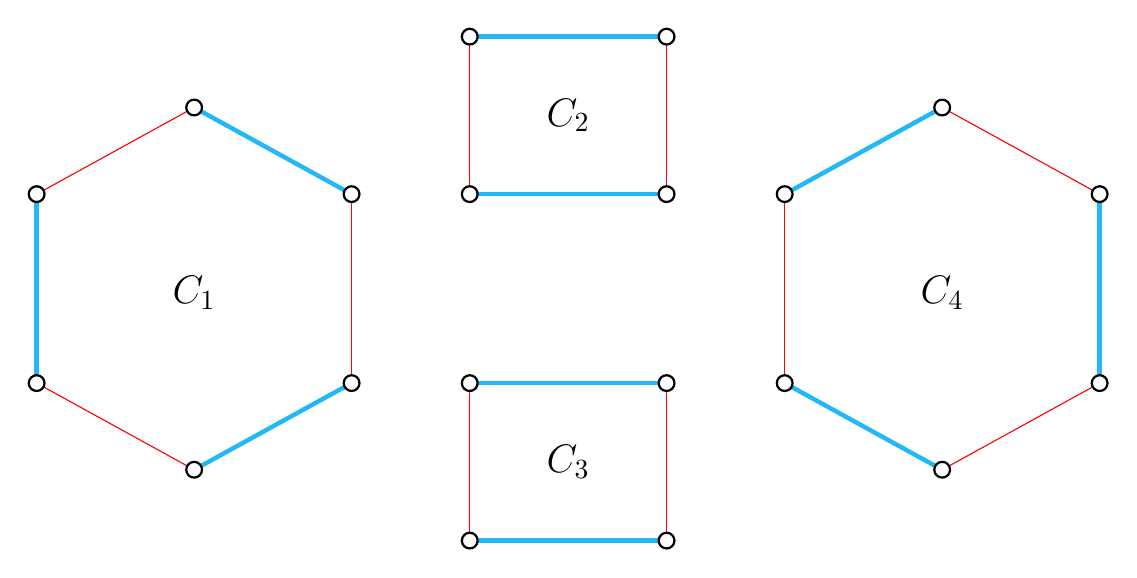
\begin{tikzpicture}
%\draw [help lines] (-1,-1) grid (20, 12);

%C1 - blue
\draw [ultra thick, tBlue] (0,2.6) -- (0,5); %v14 - v13
\draw [ultra thick, tBlue] (2,1.5) -- (4,2.6); %v3 - v1
\draw [ultra thick, tBlue] (4,5) -- (2,6.1); %v12 - v2

%C2 - blue
\draw [ultra thick, tBlue] (5.5,5) -- (8,5); %v6 - v4
\draw [ultra thick, tBlue] (5.5,7) -- (8,7); %v9 - v11

%C3 - blue
\draw [ultra thick, tBlue] (5.5,0.6) -- (8,0.6); %v10 - v7
\draw [ultra thick, tBlue] (5.5,2.6) -- (8,2.6); %v5 - v8

%C4 - blue
\draw [ultra thick, tBlue] (13.5,2.6) -- (13.5,5); %v14 - v13
\draw [ultra thick, tBlue] (11.5,1.5) -- (9.5,2.6); %v3 - v1
\draw [ultra thick, tBlue] (11.5,6.1) -- (9.5,5); %v12 - v2

%-------------------------------

%C1 - red
\draw [tRed] (0,2.6) -- (2,1.5); %v14 - v13
\draw [tRed] (4,2.6) -- (4,5); %v3 - v1
\draw [tRed] (0,5) -- (2,6.1); %v12 - v2

%C2 - red
\draw [tRed] (5.5,5) -- (5.5,7); %v6 - v4
\draw [tRed] (8,5) -- (8,7); %v9 - v11

%C3 - red
\draw [tRed] (5.5,0.6) -- (5.5,2.6); %v10 - v7
\draw [tRed] (8,0.6) -- (8,2.6); %v5 - v8

%C4 - red
\draw [tRed] (13.5,2.6) -- (11.5,1.5); %v14 - v13
\draw [tRed] (13.5,5) -- (11.5,6.1); %v3 - v1
\draw [tRed] (9.5,2.6) -- (9.5,5); %v12 - v2

%----------------------------

%C1 - vertices
\draw [fill=white, thick] (2,1.5) circle [radius = 0.1]; %v3
\draw [fill=white, thick] (0,2.6) circle [radius = 0.1]; %v12
\draw [fill=white, thick] (4,2.6) circle [radius = 0.1]; %v1
\draw [fill=white, thick] (0,5) circle [radius = 0.1]; %v2
\draw [fill=white, thick] (4,5) circle [radius = 0.1]; %v14
\draw [fill=white, thick] (2,6.1) circle [radius = 0.1]; %v13

%C2 - vertices
\draw [fill=white, thick] (5.5,5) circle [radius = 0.1]; %v6
\draw [fill=white, thick] (8,5) circle [radius = 0.1]; %v4
\draw [fill=white, thick] (5.5,7) circle [radius = 0.1]; %v9
\draw [fill=white, thick] (8,7) circle [radius = 0.1]; %v11

%C3 - vertices
\draw [fill=white, thick] (5.5,0.6) circle [radius = 0.1]; %v6
\draw [fill=white, thick] (8,0.6) circle [radius = 0.1]; %v4
\draw [fill=white, thick] (5.5,2.6) circle [radius = 0.1]; %v9
\draw [fill=white, thick] (8,2.6) circle [radius = 0.1]; %v11

%C4 - vertices
\draw [fill=white, thick] (11.5,1.5) circle [radius = 0.1]; %v3
\draw [fill=white, thick] (9.5,2.6) circle [radius = 0.1]; %v12
\draw [fill=white, thick] (13.5,2.6) circle [radius = 0.1]; %v1
\draw [fill=white, thick] (9.5,5) circle [radius = 0.1]; %v2
\draw [fill=white, thick] (13.5,5) circle [radius = 0.1]; %v14
\draw [fill=white, thick] (11.5,6.1) circle [radius = 0.1]; %v13

\node at (2,3.75) {\Large{$C_1$}};
\node at (6.75,6) {\Large{$C_2$}};
\node at (6.75,1.6) {\Large{$C_3$}};
\node at (11.5,3.75) {\Large{$C_4$}};


\end{tikzpicture}
	
\end{document}
